\documentclass{report}
\usepackage[showframe=false]{geometry}
\usepackage{titlesec}
\usepackage{amsmath}
\usepackage{graphicx}

\pagenumbering{gobble}

\geometry{tmargin=60pt,bmargin=90pt,lmargin=90pt,
rmargin=90pt}

\titleformat{\chapter}{\normalfont\huge}{\thechapter.}{20pt}{\huge}
\titlespacing*{\chapter} {0pt}{0pt}{10pt}

\begin{document}

\chapter{Section 1}

Derive the analytical solution of $w_0$ and $w_1$

\vspace{5mm}

dataset: n=1, ..., N Observations

$x_n ->$ one dimensional variable

$t_n ->$ label

linear model: $f(x_n; w_0, w_1) = w_0+w_1*x_n$

squared loss function: $L = \frac{1}{N} \sum_{N} (f(x_n) - t_n)^2$

mean value of $x_n = \overline{x}$

mean value of $t_n = \overline{t_n}$

Helpful Equation: $\sum{N} x_n = N\overline{x_n}$

Helpful Equation: $\sum{N} t_n = N\overline{t_n}$

$$L = \frac{1}{N} \sum_{N} (w_0+w_1 x_n - t_n)^2$$
\begin{equation} \label{eq1}
\begin{split}
\frac{\partial L}{\partial w_0} & = \frac{1}{N} \sum_{N} 2(w_0+w_1 x_n - t_n) \\
                                & = \frac{2}{N} \sum_{N} (w_0+w_1 x_n - t_n) = 0 \\
                                & = \frac{2}{N} (\sum_{N}w_0 + \sum_{N}w_1 x_n - \sum_{N}t_n) = 0 \\
                                & = \frac{2\sum_{N}w_0}{N} + \frac{2\sum_{N}w_1 x_n}{N} - \frac{2\sum_{N}t_n}{N} = 0 \\
                                & = \frac{2Nw_0}{N} + \frac{2w_1N\overline{x_n}}{N} - \frac{2N\overline{t_n}}{N} = 0 \\
                                & = 2w_0 + 2w_1\overline{x_n} - 2\overline{t_n} = 0
\end{split}
\end{equation}

\begin{equation} \label{eq2}
\begin{split}
\frac{\partial L}{\partial w_1} & = \frac{1}{N} \sum_{N} 2(w_0+w_1 x_n - t_n)x_n      \\
                                & = \frac{2}{N} \sum_{N} (w_0+w_1 x_n - t_n)x_n = 0 \\
                                & = \frac{2}{N} (\sum_{N}w_0 x_n + \sum_{N}w_1 x_n^2- \sum_{N}t_nx_n) = 0 \\
                                & = \frac{2}{N} (w_0\sum_{N} x_n + w_1\sum_{N} x_n^2- \sum_{N}t_nx_n) = 0 \\
                                & = \frac{2w_0\sum_{N}x_n}{N} + \frac{2w_1\sum_{N}x_n^2}{N}- \frac{2\sum_{N}t_nx_n}{N} = 0 \\
                                & = \frac{2w_0N\overline{x_n}}{N} + \frac{2w_1N\overline{x_n^2}}{N}- \frac{2N\overline{t_nx_n}}{N} = 0 \\
                                & = 2w_0\overline{x_n} + 2w_1\overline{x_n^2} - 2\overline{t_nx_n} = 0
\end{split}
\end{equation}

\begin{equation} \label{eq3}
\begin{split}
\frac{\partial L}{\partial w_0} & = 2w_0 + 2w_1\overline{x_n} - 2\overline{t_n} = 0 \\
\frac{\partial L}{\partial w_1} & = 2w_0\overline{x_n} + 2w_1\overline{x_n^2} - 2\overline{t_nx_n} = 0
\end{split}
\end{equation}

\begin{equation} \label{eq3}
\begin{split}
w_0 & = \frac{\overline{x_n}\overline{t_n} - \overline{x_nt_n}}{\overline{x_n}^2 - \overline{x_n^2}} \\
w_1 & = \overline{t_n} - \overline{x_n}\frac{\overline{x_n}\overline{t_n} - \overline{x_nt_n}}{\overline{x_n}^2 - \overline{x_n^2}}
\end{split}
\end{equation}

\chapter{Section 2}

Derive the analytical solution of $w$ in vector and matrix format

\vspace{5mm}

dataset: n=1, ..., N Observations

$W = [w_0, w_1]^T$

$X_n = [1, x_n]^T$

linear model: $f(x_n; w_0, w_1) = w_0+w_1*x_n = W^TX_n$

squared loss function: $L = \frac{1}{N} \sum_{N} (f(x_n) - t_n)^2$

$$L = \frac{1}{2N} \sum_{N} (W^TX_n - t_n)^2$$

\begin{equation} \label{eq1}
\begin{split}
L & = \frac{1}{N} \sum_{N} (W^TX_n - t_n)^2\\
  & = \frac{1}{N} (X_nW - t_n)^T(X_nW-t_n) \\
  & = ((X_nW)^T - t_n^T)(X_nW-t_n) \\
  & = (X_nW)^T X_nW - (X_nW)^Tt_n - t_n^T(X_nW) + t_n^Tt_n \\
  & = W^TX_n^TX_nW - 2(X_nW)^Tt_n + t_n^Tt_n
\end{split}
\end{equation}

\begin{equation} \label{eq2}
\begin{split}
\frac{\partial L}{\partial W}  & = 2X_n^TX_nW - 2X_n^Tt_n = 0 \\
                               & = X_n^TX_nW = X_n^Tt_n \\
                               & = (X_n^TX_n)^{-1}X_n^Tt_n
\end{split}
\end{equation}

\chapter{Section 3}
Discuss the selection of L2-norm vs L1-norm as the loss function for linear modeling (regression). You are asked to use examples of justify your answer.

When compairing L2 and L1 norms one of the biggest diffrences comes when your data contains some form of outliers. If your data does contain outliers then the L1 norm is going to move a much grater distance twards that outlier then the L2 norm would. A good example of this is shown in the figure below.

\begin{figure}[h!]
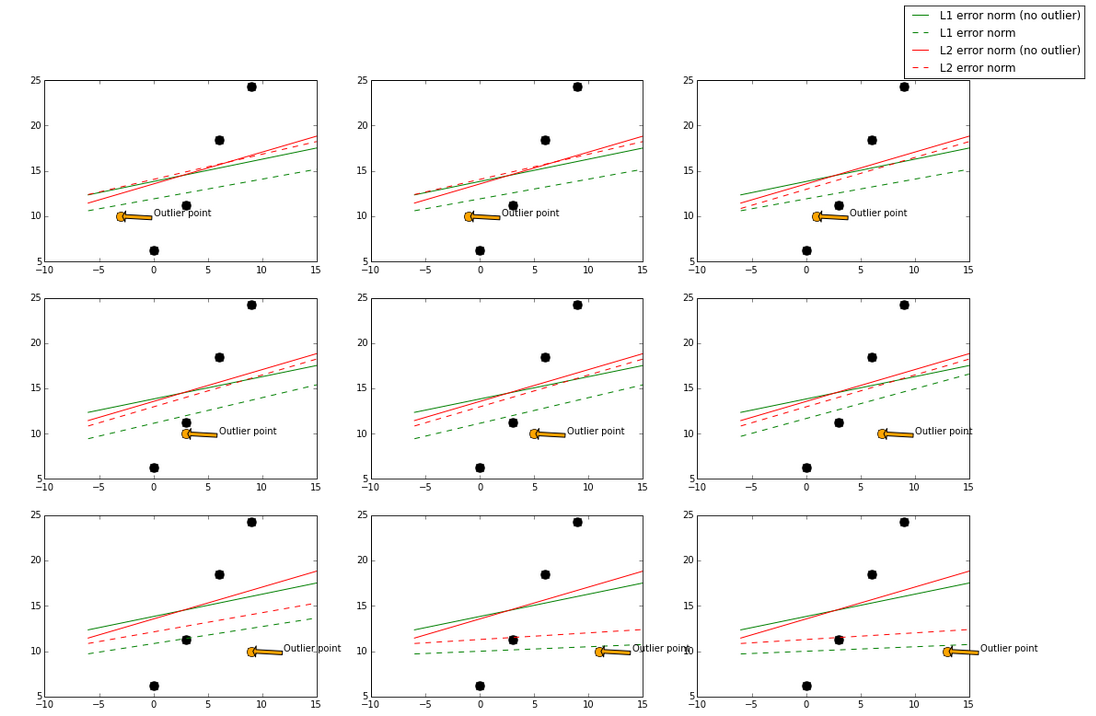
\includegraphics[width=\linewidth]{programmatic-L1-vs-L2-visualization.png}
\caption{programmatic-L1-vs-L2-visualization}
\label{fig:programmatic-L1-vs-L2-visualization}
\end{figure}

\chapter{Section 4}
S = {(1, 1), (2, 2), (3, 3)}

$$w_0 = 0$$
$$w_1 = 0$$
Step size = 0.1
$$f(x) = w_0+w_1*x_n$$

\begin{equation} \label{eq1}
\begin{split}
n & = 1\\
w_0 & = 0 + 0.1 * (1-(0+1*0)) * 1 = 0.1\\
w_1 & = 0 + 0.1 * (1-(0+1*0)) * 1 = 0.1\\
\\
n & = 2\\
w_0 & = 0.1 + 0.1 * (2-(0.1+2*0.1)) * 1 = 0.27\\
w_1 & = 0.1 + 0.1 * (2-(0.1+2*0.1)) * 2 = 0.44\\
\\
n & = 3\\
w_0 & = 0.27 + 0.1 * (3-(0.27+3*0.44)) * 1 = 0.411\\
w_1 & = 0.44 + 0.1 * (3-(0.27+3*0.44)) * 3 = 0.863\\
\\
n & = 1\\
w_0 & = 0.411 + 0.1 * (1-(0.411+1*0.863)) * 1 = 0.3836\\
w_1 & = 0.863 + 0.1 * (1-(0.411+1*0.863)) * 1 = 0.8356\\
\\
n & = 2\\
w_0 & = 0.3836 + 0.1 * (2-(0.3836+2*0.8356)) * 1 = 0.37812\\
w_1 & = 0.8356 + 0.1 * (2-(0.3836+2*0.8356)) * 2 = 0.82464\\
\\
n & = 3\\
w_0 & = 0.37812 + 0.1 * (3-(0.37812+3*0.82464)) * 1 = 0.392916\\
w_1 & = 0.82464 + 0.1 * (3-(0.37812+3*0.82464)) * 3 = 0.869028\\
\end{split}
\end{equation}

\end{document}
